\section{Evaluation}
\label{sec:evaluation} 

%We wanted to implement CORFU and we had two choices: build it from the ground
%up or do it on top of Malacology. To show the feasability of building on
%Malacology our evaluation focuses on the 

Our evaluation demonstrates the feasibility of building new service
abstractions atop programmable storage, focusing on the performance of the
internal abstractions exposed by Malacology and used to construct the Mantle
and ZLog services. We also discuss latent capabilities we discovered in this
process that let us navigate different trade-offs within the services
themselves. First, we benchmark scenarios with high sequencer contention by
examining the interfaces used to map ZLog onto Malacology; specifically, we
describe the sequencer implementation and the propagation of object and data
interfaces interfaces.  Next, we benchmark scenarios in which the storage
system manages multiple logs by using Mantle to balance sequencers across a
cluster.

% should save this for future work, otherwise it undercuts the eval.
%Detailed system-wide performance measurements and analysis is forthcoming for
%both Mantle and ZLog, as we try to find the best metadata balancing policies
%and physical design implementation trade-offs.  

Since this work focuses on the programmability of Malacology, the goal of this
section is to show that the components and subsystems that support the
Malacology interfaces provide reasonable relative performance, as well as to
give examples of the flexibility that Malacology provides to programmers.  
This section uses a principled approach for evaluating tunables of the
interfaces and the trade-offs we discuss should be acknowledged when building
higher-level services.

%As we search for the best metadata balancing policies and physical design
%implementation trade-offs, we plan to rel

\subsection{Mapping ZLog onto Malacology}
\label{sec:mapping-zlog-onto-malacology}

We evaluate Malacology by exploring one possible mapping of the ZLog
implementation of CORFU onto Ceph in which we re-use (1) the metadata service
to manage naming and synchronization of the sequencer resource by treating the
resource as an inode, and (2) the monitoring sub-subsystem to distribute and
install application-specific I/O interfaces required of the CORFU protocol. In
Section~\ref{sec:zlog-balancing} we then demonstrate how the re-use of the
inode abstraction for implementing the sequencer resource enables load
balancing policies to migrate the sequencer resource in heavy-load situation.

\subsubsection{Sequencer Implementation}
\label{sec:sequencer-implementation}

We evaluate the feasibility of using the metadata service to implement a
sequencer resource that is responsible for maintaining a total ordering of the
log. Clients contact the sequencer to obtain the tail of the log and then
independently initiate I/O, thus we measure both the throughput and latency of
obtaining new tail positions which bounds client append performance.

The sequencer is implemented using the File Type interface so that the
sequencer state (a 64-bit integer) is embedded in the inode of a file.  A total
ordering of the log is imposed by the re-use of the capability service that can
be used to grant exclusive access of inode state to clients. The metadata
service is responsible for maintaining exclusivity and granting access.
Figure~\ref{fig:capdelay-quota-behavior} (a) shows the behavior of the system
in which a best-effort policy is used.  The two colors represent points in time
that the clients were able to access the resource.  The best-effort policy
shows a high degree of interleaving between clients but the system spends a
large portion of time re-distributing the capability, reducing overall
throughput.

In order to control the performance of the system we implement a policy that
(1) restricts the length of time that a client may maintain exclusive access
and (2) limits the number of log positions that a client may generate without
yielding to other clients waiting for access. The behavior of these two modes
is illustrated in Figures~\ref{fig:capdelay-quota-behavior} (b) and (c),
respectively.

\begin{figure}[tbp]
\centering
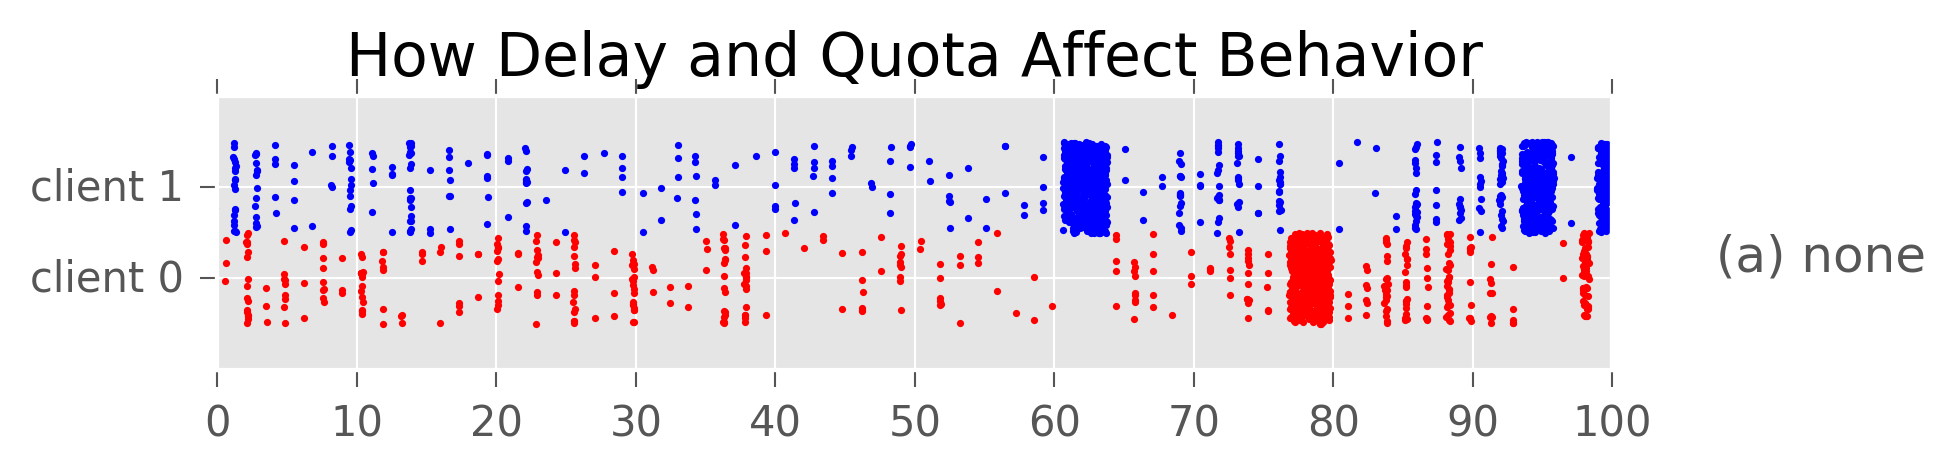
\includegraphics{figures/capdelay-quota-behavior-a.png}
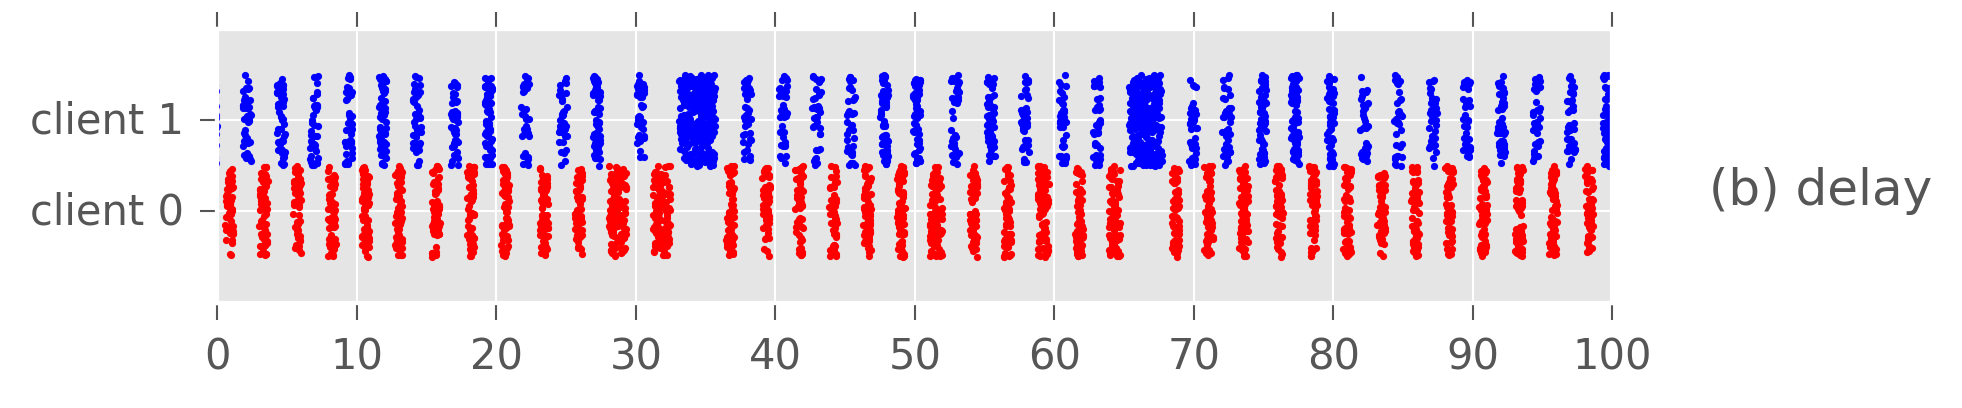
\includegraphics{figures/capdelay-quota-behavior-b.png}
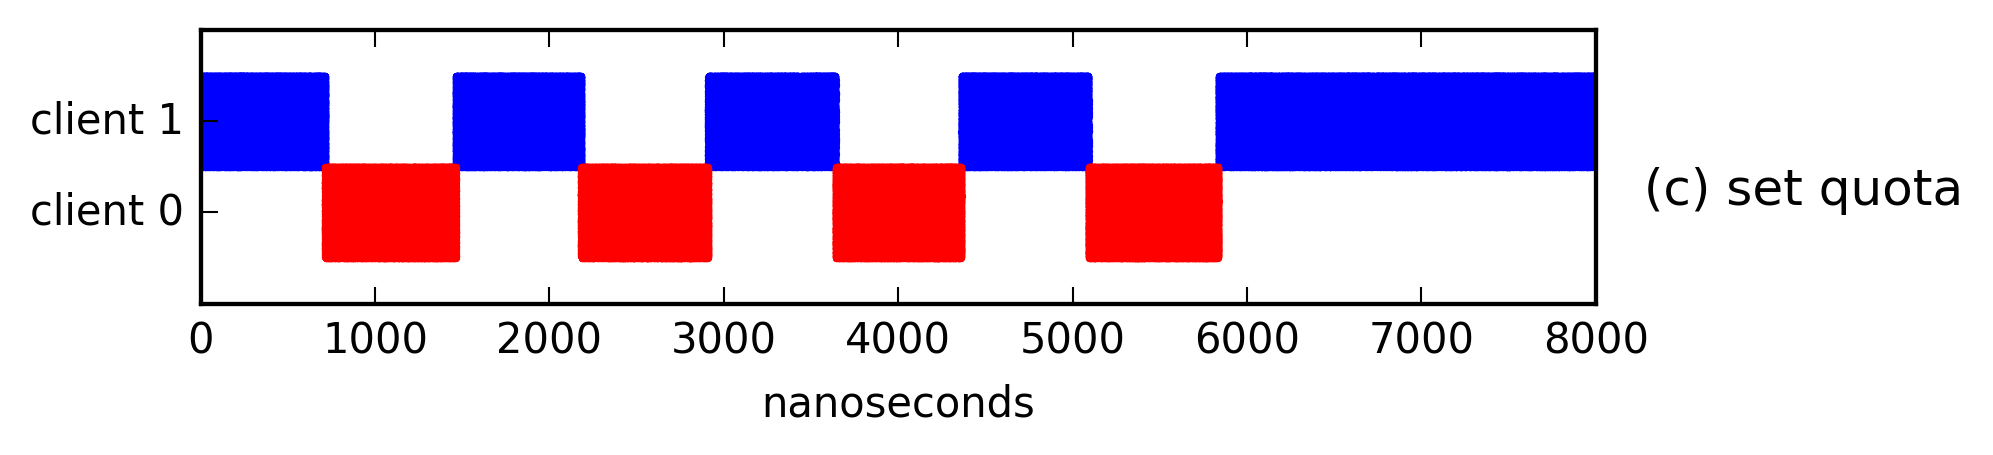
\includegraphics{figures/capdelay-quota-behavior-c.png}
\caption{
[\href{https://github.com/michaelsevilla/malacology-popper/blob/v2.1/experiments/mds-zlog-seq-thruput-v-latency/results-reqdots-kill0-sameclient-capdelay-100-quota-100000/visualize.ipynb}{source}]
Each dot is an individual request, spread randomly along the \(y\) axis. The
default behavior is unpredictable, ``delay" lets clients hold the lease longer,
and ``quota" gives clients the lease for a number of operations.}
\label{fig:capdelay-quota-behavior}
\end{figure}

Figure~\ref{fig:captp} demonstrates a configurable trade-off between throughput
and latency. In the experiment two clients are run each with a fixed 0.25
second maximum reservation on the capability, and we vary the size of the log
position quota running each configuration for two minutes. The total operations
per second is the combined throughput of the two clients, and the average
latency is the number of microseconds required to obtain a new log position. With a
small quota more time is spent exchanging exclusive access, while a large quota
reservation allows clients to experience a much lower latency because they
experience isolated access for a longer period of time.

\begin{figure}[tbp]
\centering
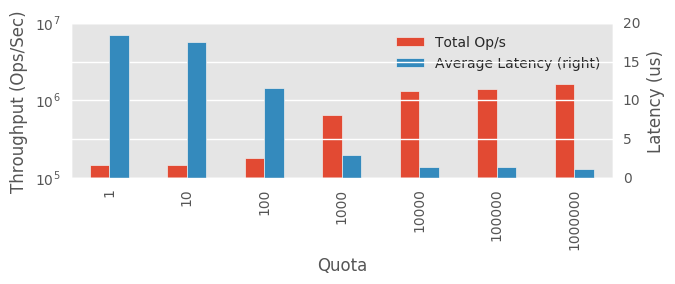
\includegraphics{figures/tradeoff.png}
\caption{
[\href{https://github.com/michaelsevilla/malacology-popper/blob/v2.1/experiments/zlog-seqr-redux/viz.ipynb}{source}]
Sequencer throughput by re-using various services.  The highest performance is
achieved using a single client with exclusive, cacheable privilege. Round-robin
sharing of the sequencer resource is affected by the amount of time the
resource is held, with best-effort performing the worst.}
\label{fig:captp}
\end{figure}

To get a better picture of latency, Figure~\ref{fig:capcdf} shows the CDF of
latency for each client in all experiment configurations. At the 99th
percentile clients accessed the sequencer in less than a millisecond. The CDF
is cropped at the 99.999th percentile due to large outliers that we believe
occur in instances in which the metadata server is performing I/O while it is in the
process of re-distributing the capability to another client.

\begin{figure}[tbp]
\centering
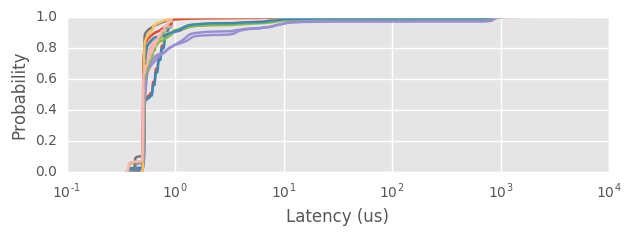
\includegraphics{figures/caps-delay-latency.png}
\caption{
[\href{https://github.com/michaelsevilla/malacology-popper/blob/v2.1/experiments/zlog-seqr-redux/viz.ipynb}{source}]
The latency distribution shows that if the clients hold their capabilities
longer, performance decreases. Changing the delay can help the sequencer and
clients strike a balance between throughput and latency.}
\label{fig:capcdf}
\end{figure}

\textbf{Malacology exposes} the internal capability management service and
allows users to navigate latency and throughput trade-offs.  Other approaches
to designing the sequencer service also exist, such as using a centralized
service in which each access is a network round-trip. In contrast to the
mechanism we explored which is appropriate for clients with bursty workloads,
it may be easier to provide predictable performance using a centralized
service, and we will be exploring in the future how this can be achieved using
the capability system.

\subsubsection{Interface Propagation}

Domain-specific data interfaces
(Section~\ref{sec:application-specifc-storage-stacks}) allow co-design between
applications and the storage system. Malacology supports custom object
interfaces in RADOS that require interface implementations to be installed on
the storage devices in the system, supporting the evolution of interfaces
through automatic system-wide versioning and installation through the service
metadata interface (Section~\ref{service-metadata}). We evaluate the
performance of installing a new interface version in the cluster, which is an
important metric for applications that frequently evolve interfaces.

We demonstrate the feasibility of utilizing the Ceph monitoring sub-system by
evaluating the performance of installing and distributing interface updates.
Figure~\ref{fig:propdelay} shows the CDF of the latency of interface updates.
The interfaces are Lua scripts embedded in the cluster map and distributed
using a peer-to-peer gossip protocol.  The latency is defined as the elapsed
time following the Paxos proposal for an interface update until each object
storage daemon makes the update live (the cost of the Paxos proposal is
configurable and is discussed below). The latency measurements were taken on
the nodes running object server daemons, and thus exclude the client round-trip
cost. In each of the experiments 1000 interface updates were observed.

Figure~\ref{fig:propdelay} shows the lower bound cost for updates in a large
cluster. In the experiment labeled ``120 OSD (RAM)" a cluster of 120 object
storage daemons (OSDs) using an in-memory data store were deployed, showing a
latency of less than 54 ms with a probability of 90\% and a worst case latency
of 194 ms. These costs demonstrate the penalty of distributing the interface in
a large cluster. In practice the costs include, in addition to cluster-wide
propagation of interface updates, the network round-trip to the interface
management service, the Paxos commit protocol itself, and other factors such as
system load. By default Paxos proposals occur periodically with a 1 second
interval in order to accumulate updates. In a minimum, realistic quorum of 3
monitors using hard drive-based storage, we were able to decrease this interval
to an average of 222 ms.

\begin{figure}[tbp]
\centering
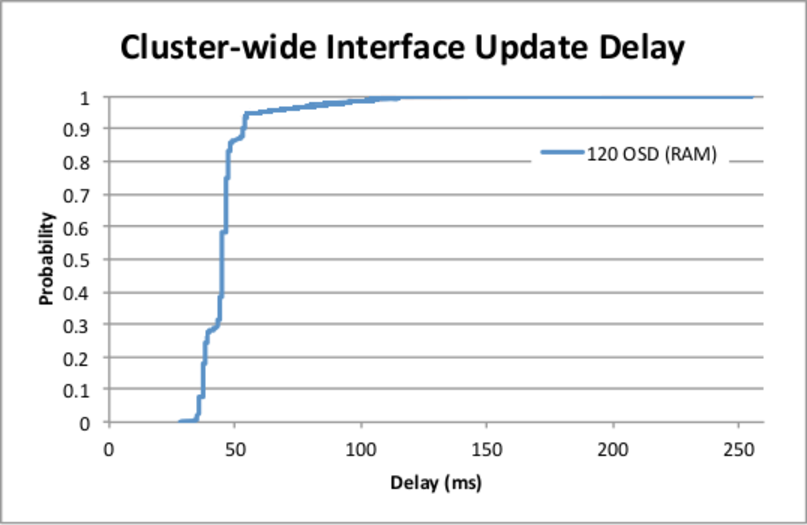
\includegraphics[width=60mm,trim={1 4 4 1.3cm},clip]{figures/iface-update-delay.pdf}
\caption{
[\href{https://github.com/michaelsevilla/malacology-popper/tree/v2.1/experiments/mon-paxos-update/viz.py}{source}]
Cluster-wide interface update latency, excluding the Paxos proposal cost for
committing the Service Metadata interface.}
\label{fig:propdelay}
\end{figure}

\subsection{Load Balancing ZLog Sequencers with Mantle}
\label{sec:zlog-balancing}

In practice, a storage system implementing CORFU will support a multiplicity of
independent totally-ordered logs for each application.  For this scenario
co-locating sequencers on the same physical node is not ideal but building a
load balancer that can migrate the shared resource (e.g., the resource
that mediates access to the tail of the log) is a time-consuming, non-trivial
task.  It requires building subsystems for migrating resources, monitoring the
workloads, collecting metrics that describe the utilization on the physical
nodes, partitioning resources, maintaining cache coherence, and managing
multiple sequencers. The following experiments demonstrate the feasibility of
using the mechanisms of the Malacology Load Balancing interface to inherit
these features and to alleviate load from overloaded servers.

\begin{figure}[t!]
\centering
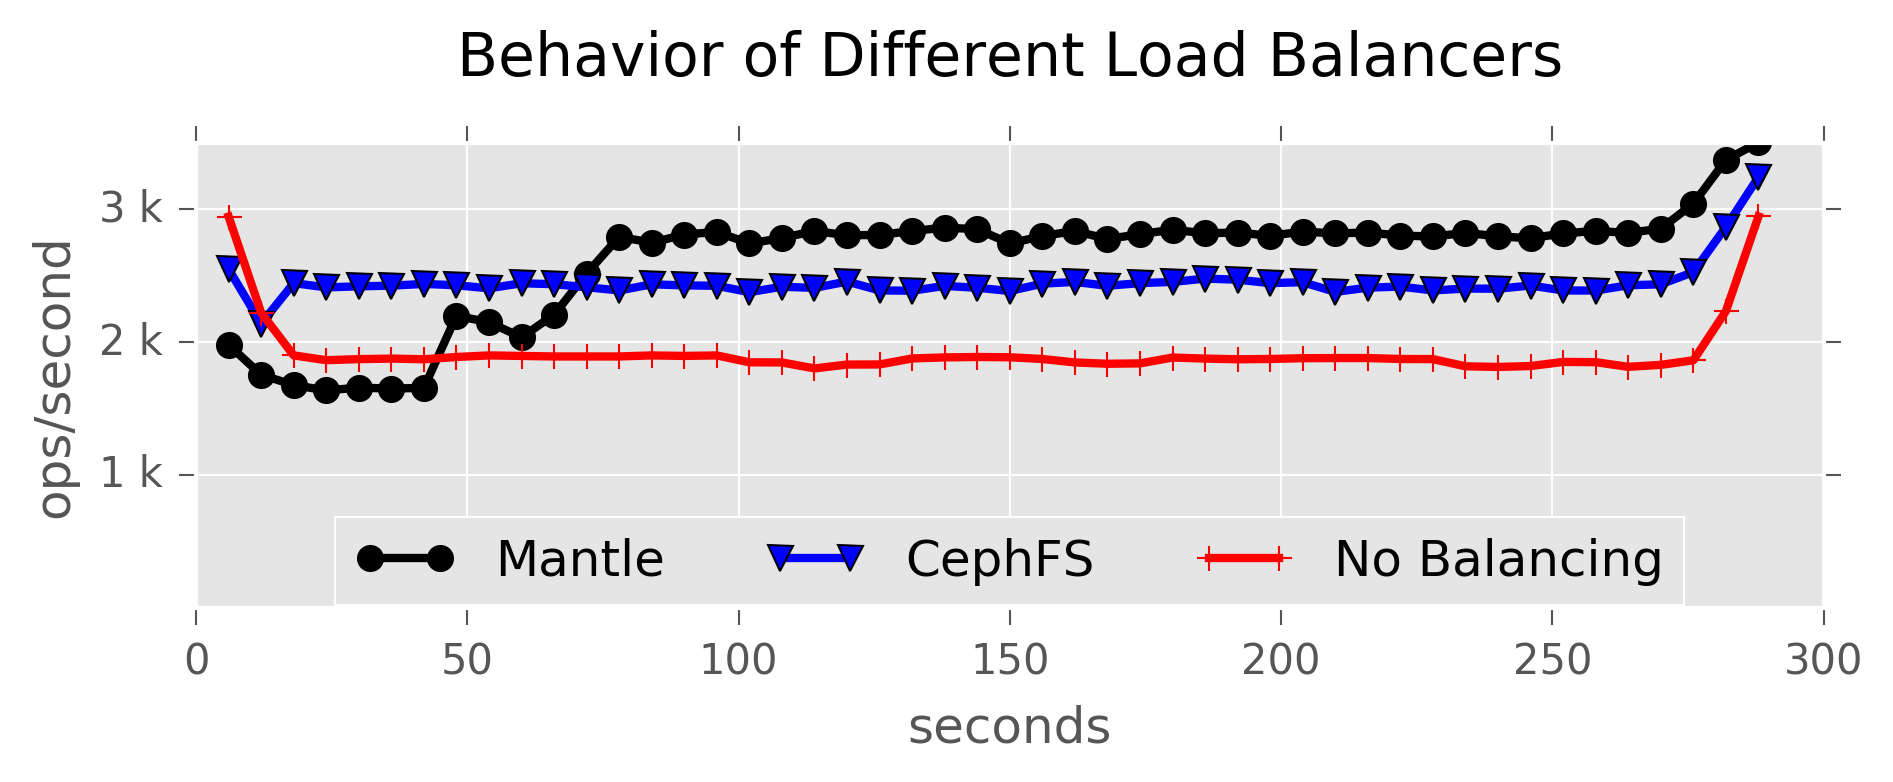
\includegraphics{figures/mantle-balancer-behaviors.png}
\caption{
[\href{https://github.com/michaelsevilla/malacology-popper/blob/v2.1/experiments/mds-zlog-seq-migrate-redux-3client/results-mantle-runs/visualize.ipynb}{source}]
CephFS/Mantle load balancing have better throughput than co-locating all
sequencers on the same server.  Sections~\ref{sec:feature-balancing-modes}
and~\ref{sec:feature-migration-units} quantify this improvement;
Section~\ref{sec:feature-backoff} examines the migration at 0-60 seconds.
}\label{fig:mantle-balancer-behaviors}
\end{figure}

\begin{figure}[t!]
\centering
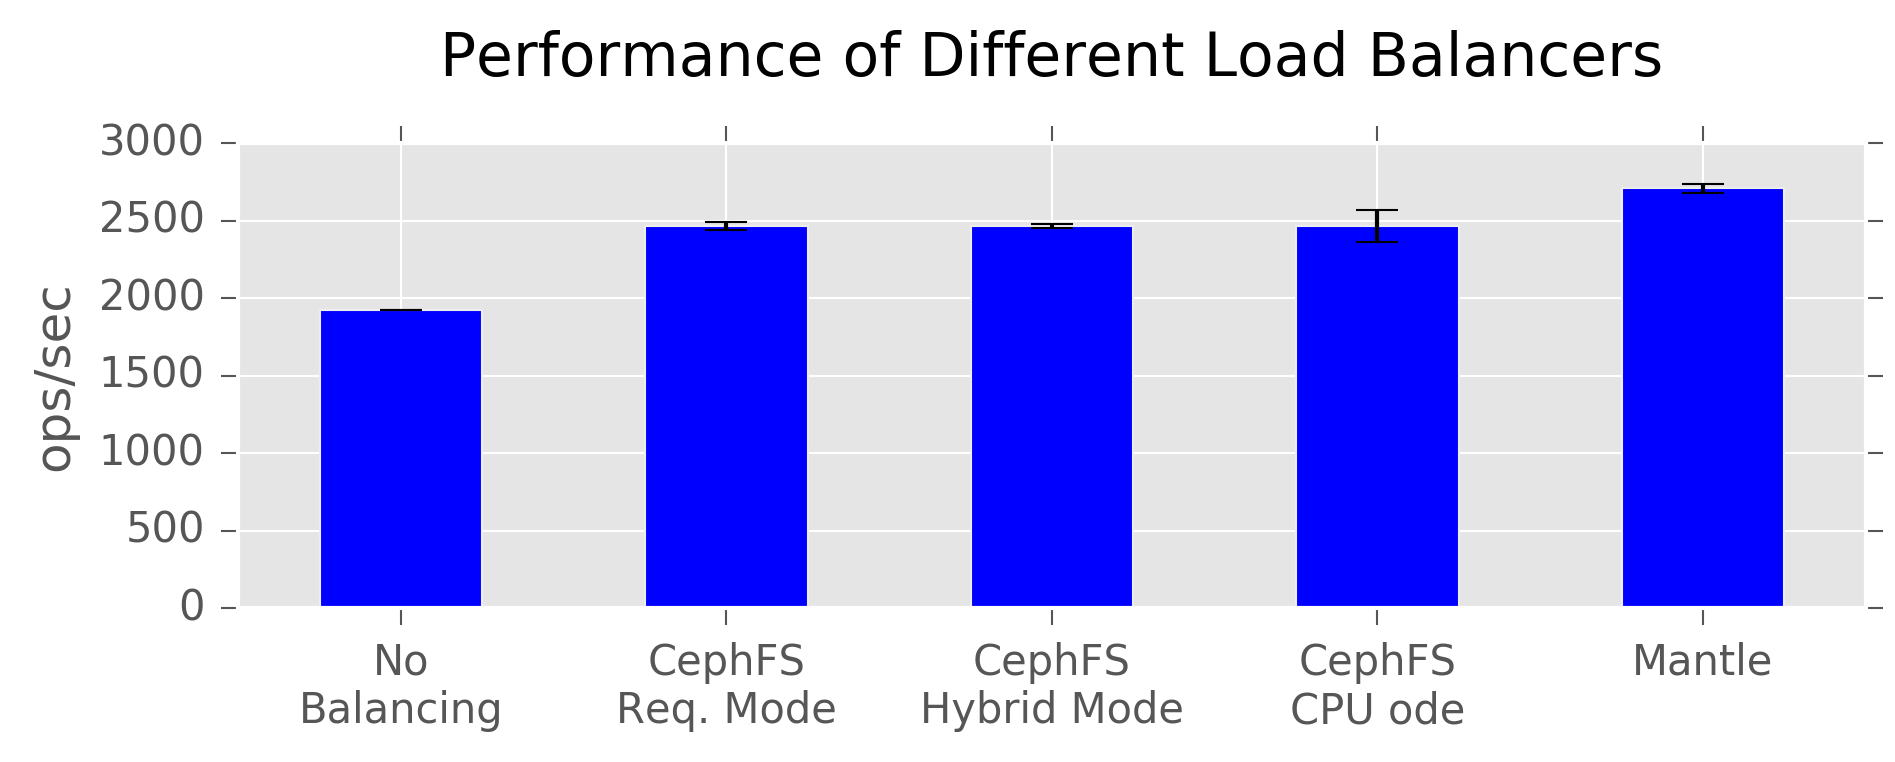
\includegraphics{figures/mantle-balancer-performance.png}
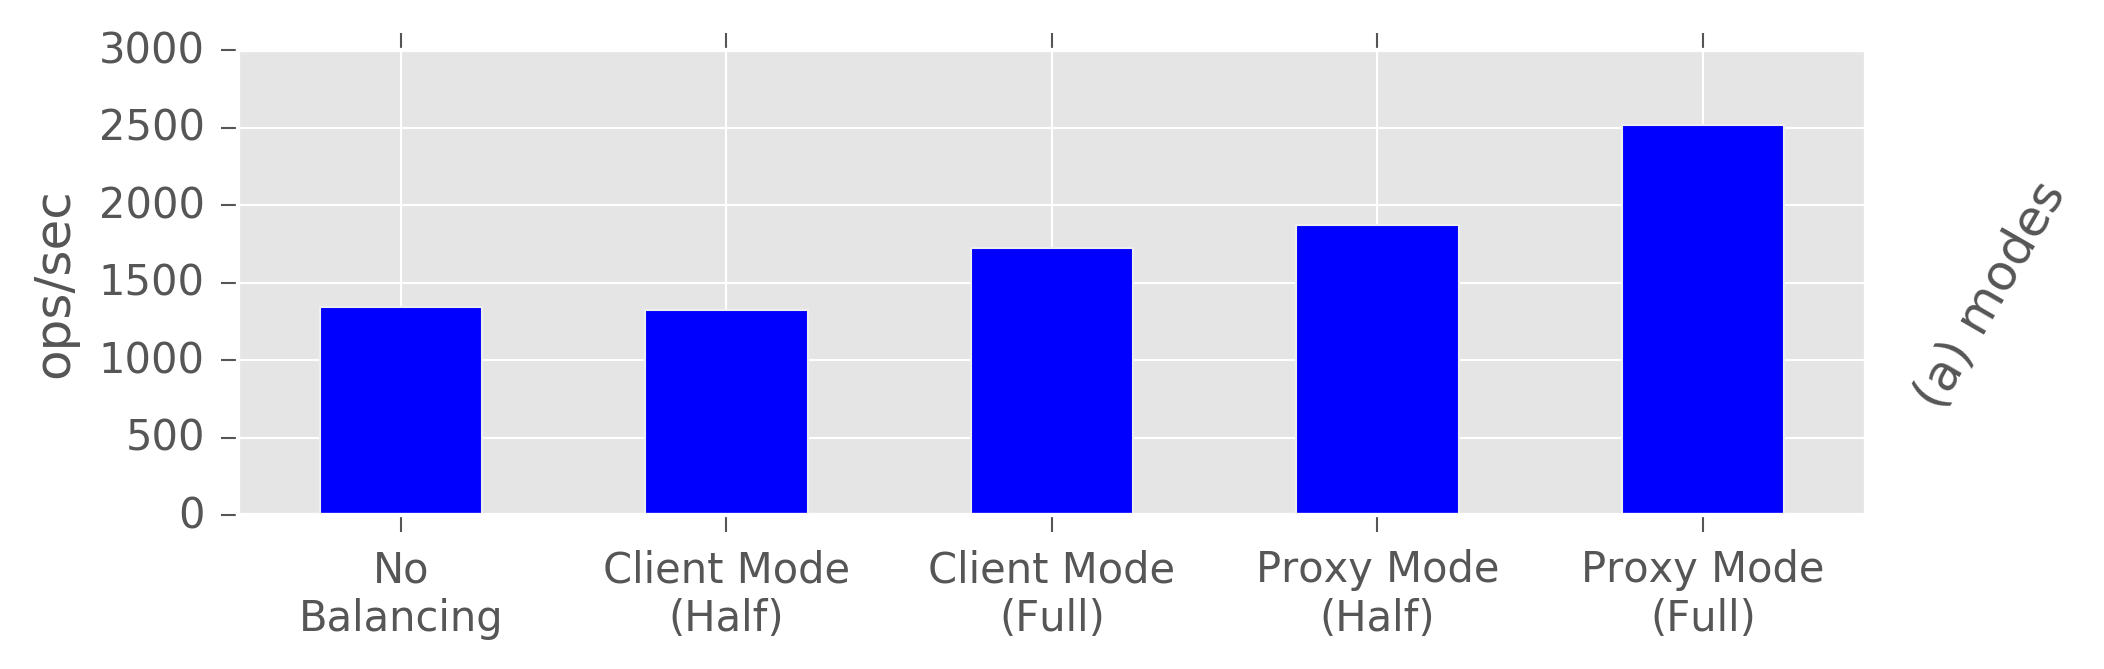
\includegraphics{figures/mantle-mode-performance.png}
\caption{
[\href{https://github.com/michaelsevilla/malacology-popper/blob/v2.1/experiments/mds-zlog-seq-migrate-redux-3client/results-mantle-runs/visualize.ipynb}{source},
\href{https://github.com/michaelsevilla/malacology-popper/blob/v2.1/experiments/mds-zlog-seq-migrate-redux-waves/results-paper/visualize.ipynb}{source}]
In (a) all CephFS balancing modes have the same performance; Mantle uses a
balancer designed for sequencers. In (b) the best combination of mode and
migration units can have up to a 2\(\times\)
improvement.}\label{fig:mantle-balancer-performance}
\end{figure}

The experiments are run on a cluster with 10 nodes to store objects, one node
to monitor the cluster, and 3 nodes that can accommodate sequencers.  Instead
of measuring contention at the clients like
Section~\ref{sec:sequencer-implementation}, these experiments measure
contention at the sequencers by forcing clients to make round-trips for every
request. We implement this using the Shared Resource interface that forces
round-trips.  Because the sequencer's only function is to  hand out positions
for the tail of the log, the workload is read-heavy.

First, we show how the ZLog service can orchestrate multiple sequencers using
the Malacology Load Balancing interface.
Figure~\ref{fig:mantle-balancer-behaviors} shows the throughput over time of
different load balancers as they migrate 3 sequencers (with 4 clients) around
the cluster; ``No Balancing" keeps all sequencers on one server, ``CephFS"
migrates sequencers using the hard-coded CephFS load balancers, and ``Mantle"
uses a custom load balancer we wrote specifically for sequencers.  The
increased throughput for the CephFS and Mantle curves between 0 and 60 seconds
are a result of migrating the sequencer(s) off overloaded servers.

In addition to showing that migrating sequencers improves performance,
Figure~\ref{fig:mantle-balancer-behaviors} also demonstrates features that we
will explore in the rest of this section.
Sections~\ref{sec:feature-balancing-modes}
and~\ref{sec:feature-migration-units} quantify the differences in performance
when the cluster stabilizes at time 100 seconds and
Section~\ref{sec:feature-backoff} examines the slope and start time of the
re-balancing phase between 0 and 60 seconds by comparing the aggressiveness of
the balancers.

\subsubsection{Feature: Balancing Modes}
\label{sec:feature-balancing-modes}

Next, we quantify the performance benefits shown in
Figure~\ref{fig:mantle-balancer-behaviors}.  To understand why load balancers
perform differently we need to explain the different balancing modes that the
load balancer service uses and how they stress the subsystems that receive and
forward client requests in different ways. In
Figure~\ref{fig:mantle-balancer-behaviors}, the CephFS curve shows the
performance of the balancing mode that CephFS falls into {\it most of the
time}.  CephFS currently has 3 modes for balancing load: CPU mode, workload
mode, and hybrid mode. All three have the same structure for making migration
decisions but vary based on the metric used to calculate load. For this
sequencer workload the 3 different modes all have the same performance, shown
in Figure~\ref{fig:mantle-balancer-performance} (a), because the load balancer
falls into the same mode a majority of the time.  The high variation in
performance for the CephFS CPU Mode bar reflects the uncertainty of using
something as dynamic and unpredictable as CPU utilization to make migration
decisions.  In addition to the suboptimal performance and unpredictability,
another problem is that all the CephFS balancers behave the same. This prevents
administrators from properly exploring the balancing state space.

Mantle gives the administrator more control over balancing policies; for the
Mantle bar in Figure~\ref{fig:mantle-balancer-performance} (a) we use the Load
Balancing interface to program logic for balancing read-heavy workloads,
resulting in better throughput and stability.  When we did this we also
identified two balancing modes relevant for making migration decisions for
sequencers. 

Using Mantle, the administrator can put the load balancer into ``proxy mode" or
``client mode". In proxy mode one server receives all requests and farms off
the requests to slave servers; the slave servers do the actual tail finding
operation. In client mode, clients interact directly with the server that has
their sequencer.  These modes are illustrated in Figure~\ref{fig:mantle-modes}.
``No Balancing" is when all sequencers are co-located on one physical server --
performance for that mode is shown by the ``No Balancing" curve in
Figure~\ref{fig:mantle-balancer-behaviors}. In ``Proxy Mode", clients continue
sending requests to server A even though some of the sequencers have been
migrated to another server. Server A redirects client requests for sequencer 2
to server B.  ``Proxy Mode (Half)" is shown in
Figure~\ref{fig:mantle-balancer-behaviors}; in this scenario, half of the
sequencers have migrated off the first server. Alternatively, ``Proxy Mode
(Full)", which is not pictured, is when all the sequencers migrate off the
first server.  ``Client Mode", shown on the far right of
Figure~\ref{fig:mantle-modes}, shows how clients for sequencer 2 contact server
B without a redirect from server A.

\begin{figure}[t!]
\centering
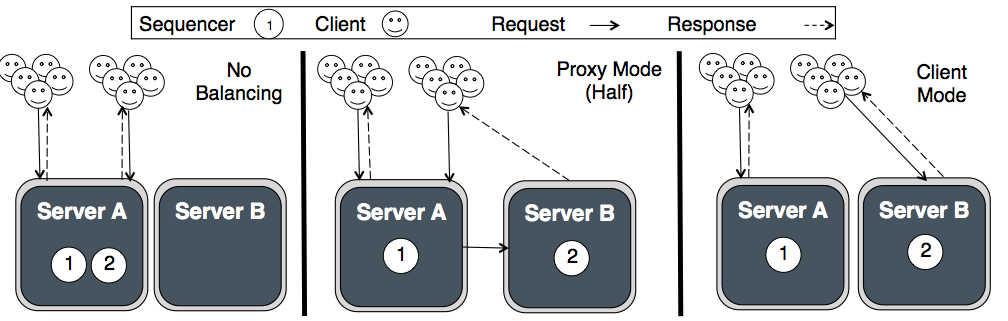
\includegraphics{figures/mantle-modes.png}
\caption{ In client mode clients sending requests to the server that houses
their sequencer. In proxy mode clients continue sending their requests to the
first server.  }\label{fig:mantle-modes}
\end{figure}

\begin{figure}[t!]
\centering
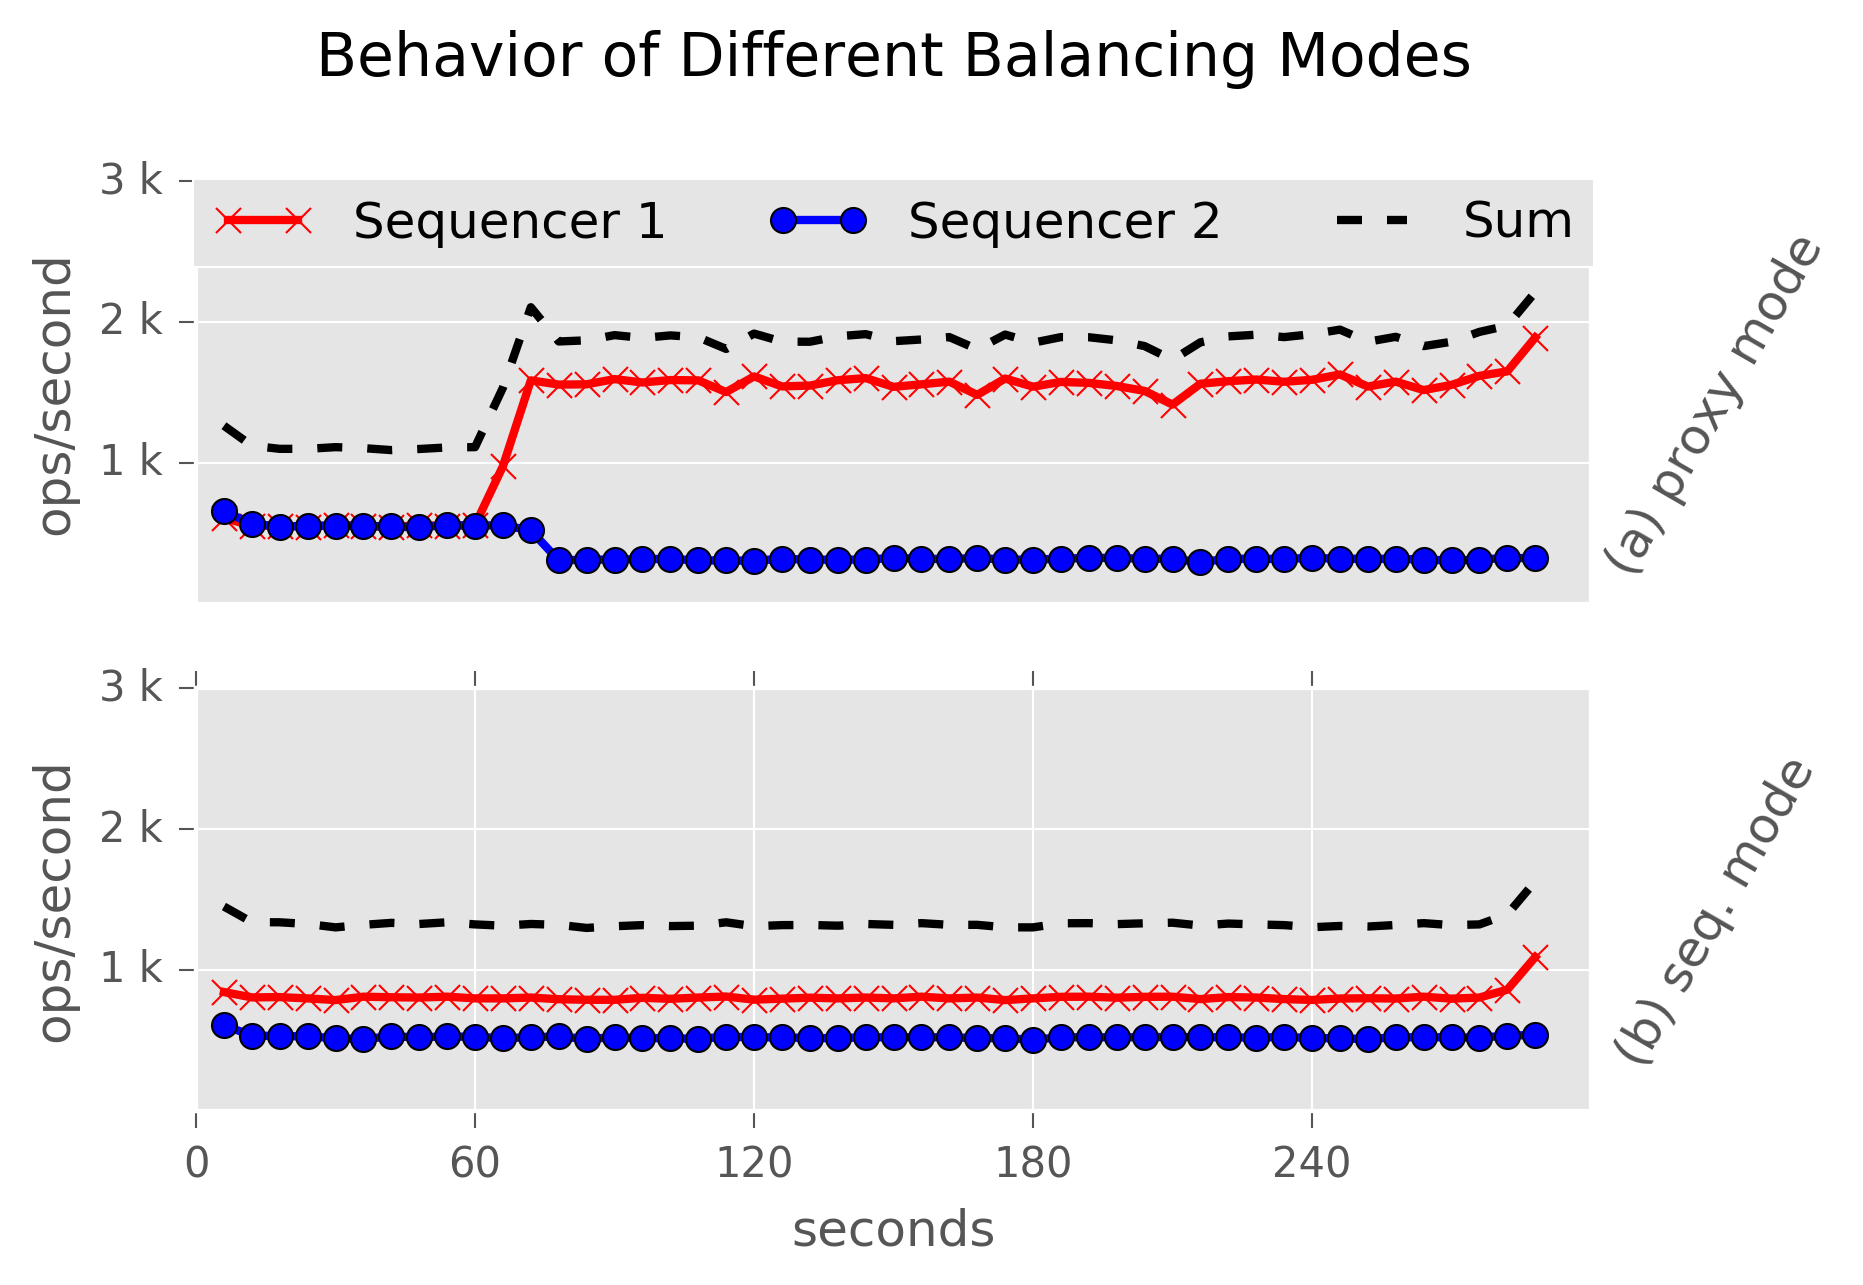
\includegraphics{figures/mantle-mode-behavior.png}
\caption{
[\href{https://github.com/michaelsevilla/malacology-popper/blob/v2.1/experiments/mds-zlog-seq-migrate-redux-waves/results-paper/visualize.ipynb}{source}]
The performance of proxy mode achieves the highest throughput but at the cost
of lower throughput for one of the sequencers. Client mode is more fair but
results in lower cluster throughput.  }\label{fig:mantle-mode-behavior}
\end{figure}

Figure~\ref{fig:mantle-mode-behavior} shows the throughput over time of the two
different modes for an environment with only 2 sequencers (again 4 clients
each) and 2 servers. The curves for both sequencers in
Figure~\ref{fig:mantle-mode-behavior}(a) start at less than 1000 ops/second and
at time 60 seconds Mantle migrates Sequencer 1 to the slave server.
Performance of Sequencer 2 decreases because it stayed on the proxy which now
processes requests for Sequencer 2, and forwards requests for Sequencer 1. The
performance of Sequencer 1 improves dramatically because distributing the
sequencers in this way separates (1) the handling of the client requests and
(2) finding the tail of the log and responding to clients.  Doing both steps is
too heavy weight for one server and sequencers on slave nodes can go faster if
work is split up; this phenomenon is not uncommon and has been observed in
chain replication~\cite{chain_rep}.

Cluster throughput improves at the cost of decreased throughput for Sequencer
2.  Figure~\ref{fig:mantle-mode-behavior}(b) is set to sequencer mode manually
(no balancing phase) and shows that the cluster throughput is worse than the
cluster throughput of proxy mode. That graph also shows that Sequencer 2 has
less throughput than Sequencer 1. In this case, the scatter-gather process used
for cache coherence in the metadata protocols causes strain on the server
housing Sequencer 2 resulting in this uneven performance. 

\subsubsection{Feature: Migration Units}
\label{sec:feature-migration-units}

Another factor that affects performance in this environment is how much load is
on each server; these experiments quantify that effect by programming the Load
Balancing interface to control the amount of load to migrate. We call this
metric a ``migration unit".  Expressing this heuristic is not easily achievable
with outward facing tunable parameters (i.e. system knobs) but with Mantle's
programmable interface, we can force the load balancer to change its migration
units. To force the balancer into the Proxy Mode (Half) scenario in
Figure~\ref{fig:mantle-modes}, which uses migration units equal to half the
load on the current server, we can use: \texttt{ targets[whoami+1] =
mds[whoami]["load"]/2 }.

This code snippet uses globally defined variables and tables from the Mantle
API~\cite{sevilla:sc15-mantle} to send half of the load on the current server
(whoami) to the next ranked server (whoami + 1); the \texttt{targets} array is
a globally defined table that the balancer uses to do the migrations.
Alternatively, to migrate all load a time step, we can remove the division by
2.

%\begin{figure}[t!]
%\centering
%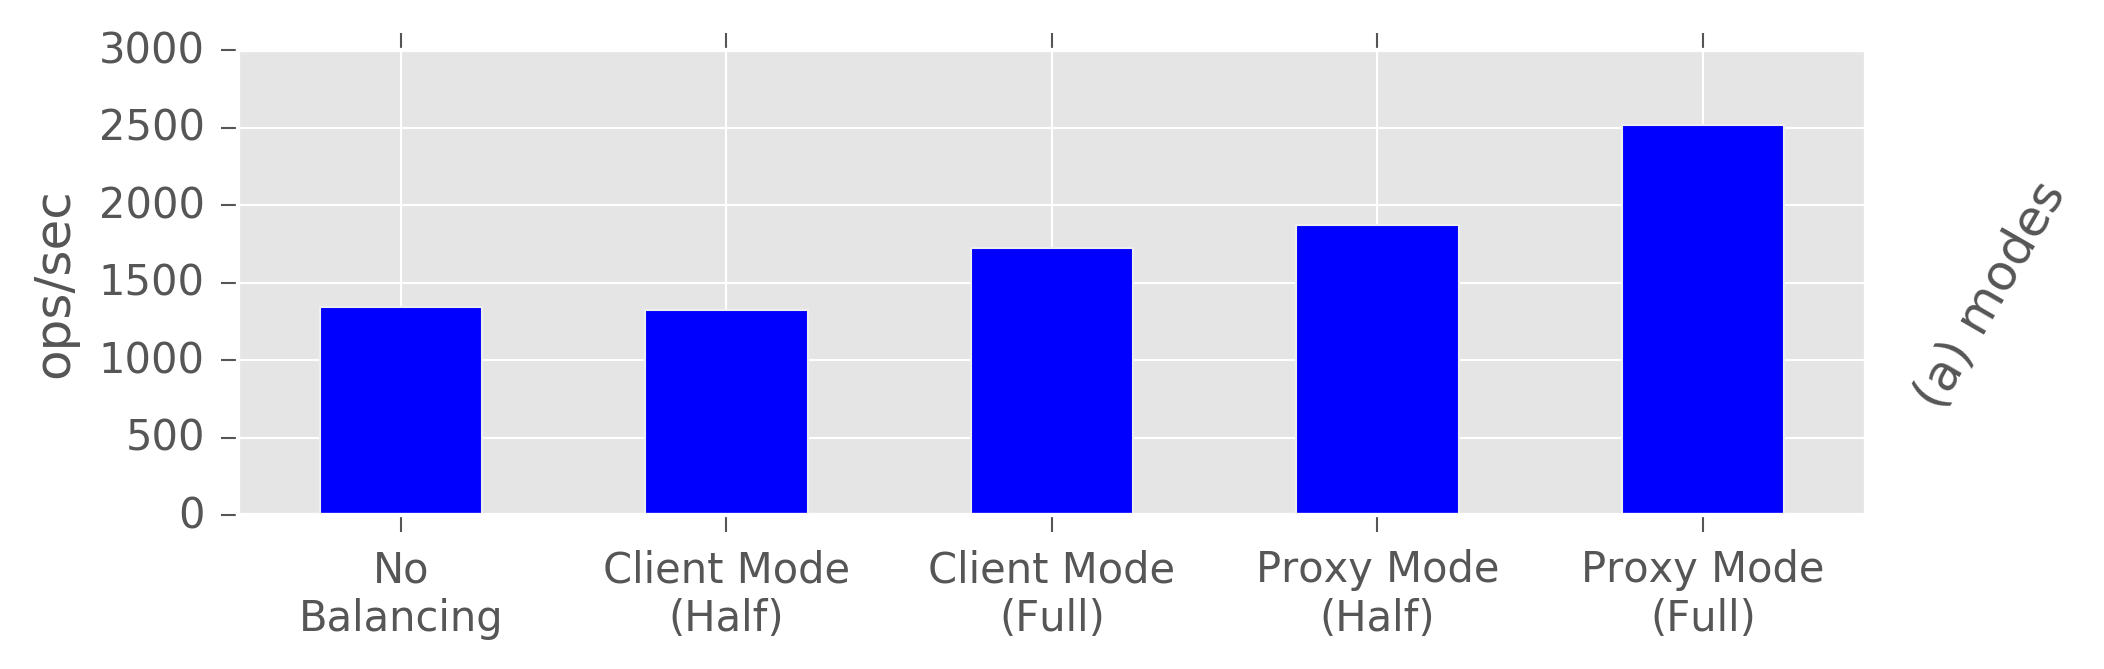
\includegraphics{figures/mantle-mode-performance.png}
%\caption{The performance of the different modes using various migration units
%shows almost a 2\(\times\) improvement in the best case.
%}\label{fig:mantle-mode-performance}
%\end{figure}

Figure~\ref{fig:mantle-balancer-performance} (b) shows the performance of the
modes using different migration units. Recall that this setup only has 2
sequencers and 2 servers, so performance may be different at scale. Even so, it
is clear that client mode does not perform as well for read-heavy workloads. We
even see a throughput improvement when migrating all load off the first server,
leaving the first server to do administrative tasks (this is common in the
metadata cluster because the first server does a lot of the cache coherence
work) while the second server does all the processing. Proxy mode does the
best in both cases and shows large performance gains when completely decoupling
client request handling and operation processing in Proxy Mode (Full).  The
parameter that controls the migration units helps the administrator control the
sequencer co-location or distribution across the cluster. This trade-off was
explored extensively in the Mantle paper but the experiments we present here
are indicative of an even richer set of states to explore.

\subsubsection{Feature: Backoff}
\label{sec:feature-backoff}

Tuning the aggressiveness of the load balancer decision making is also a
trade-off that administrators can control and explore. The balancing phase from
0 to 60 seconds in Figure~\ref{fig:mantle-balancer-behaviors} shows different
degrees of aggressiveness in making migration decisions; CephFS makes a
decision 10 seconds into the run and throughput jumps to 2500 ops/second 
while Mantle takes more time to stabilize. This conservative behavior is
controlled by programming the balancer to (1) use different conditions for when
to migrate and (2) using a threshold for sustained overload. 

We control the conditions for when to migrate using \texttt{when()}, a callback
in the Mantle API.  For the Mantle curve in
Figure~\ref{fig:mantle-balancer-behaviors} we program \texttt{when()} to wait
for load on the receiving server to fall below a threshold. This makes the
balancer more conservative because it takes 60 seconds for cache coherence
messages to settle.  The Mantle curve in
Figure~\ref{fig:mantle-balancer-behaviors} also takes longer to reach peak
throughput because we want the policy to wait to see how migrations affect the
system before proceeding; the balancer does a migration right before 50
seconds, realizes that there is a third underloaded server, and does another
migration. 

The other way to change aggressiveness of the decision making is to program
into the balancer a threshold for sustained overload. This forces the balancer
to wait a certain number of iterations after a migration before proceeding. In
Mantle, the policy would use the save state function to do a countdown after a
migration.  Behavior graphs and performance numbers for this backoff feature is
omitted for space considerations, but our experiments confirm that the more
conservative the approach the less overall throughput.
 
\textbf{Malacology pulls} the load balancing service out of the storage system
to balance sequencers across a cluster. This latent capability also gives
future programmers the ability to explore the different load balancing
trade-offs including: load balancing modes to control forwarding vs. client
redirection, load migration units to control sequencer distribution vs.
co-location, and backoffs to control conservative vs. aggressive decision
making.

%\subsubsection{Experiment: Object Class
%Programmability}\label{experiment-object-class-programmability}
%
%Add quote from CORFU paper that talks about what they had to hack
%
%\subsubsection{Experiment: Multi-Client
%Burstiness}\label{experiment-multi-client-burstiness}
%
%\begin{figure}[htbp] \centering
%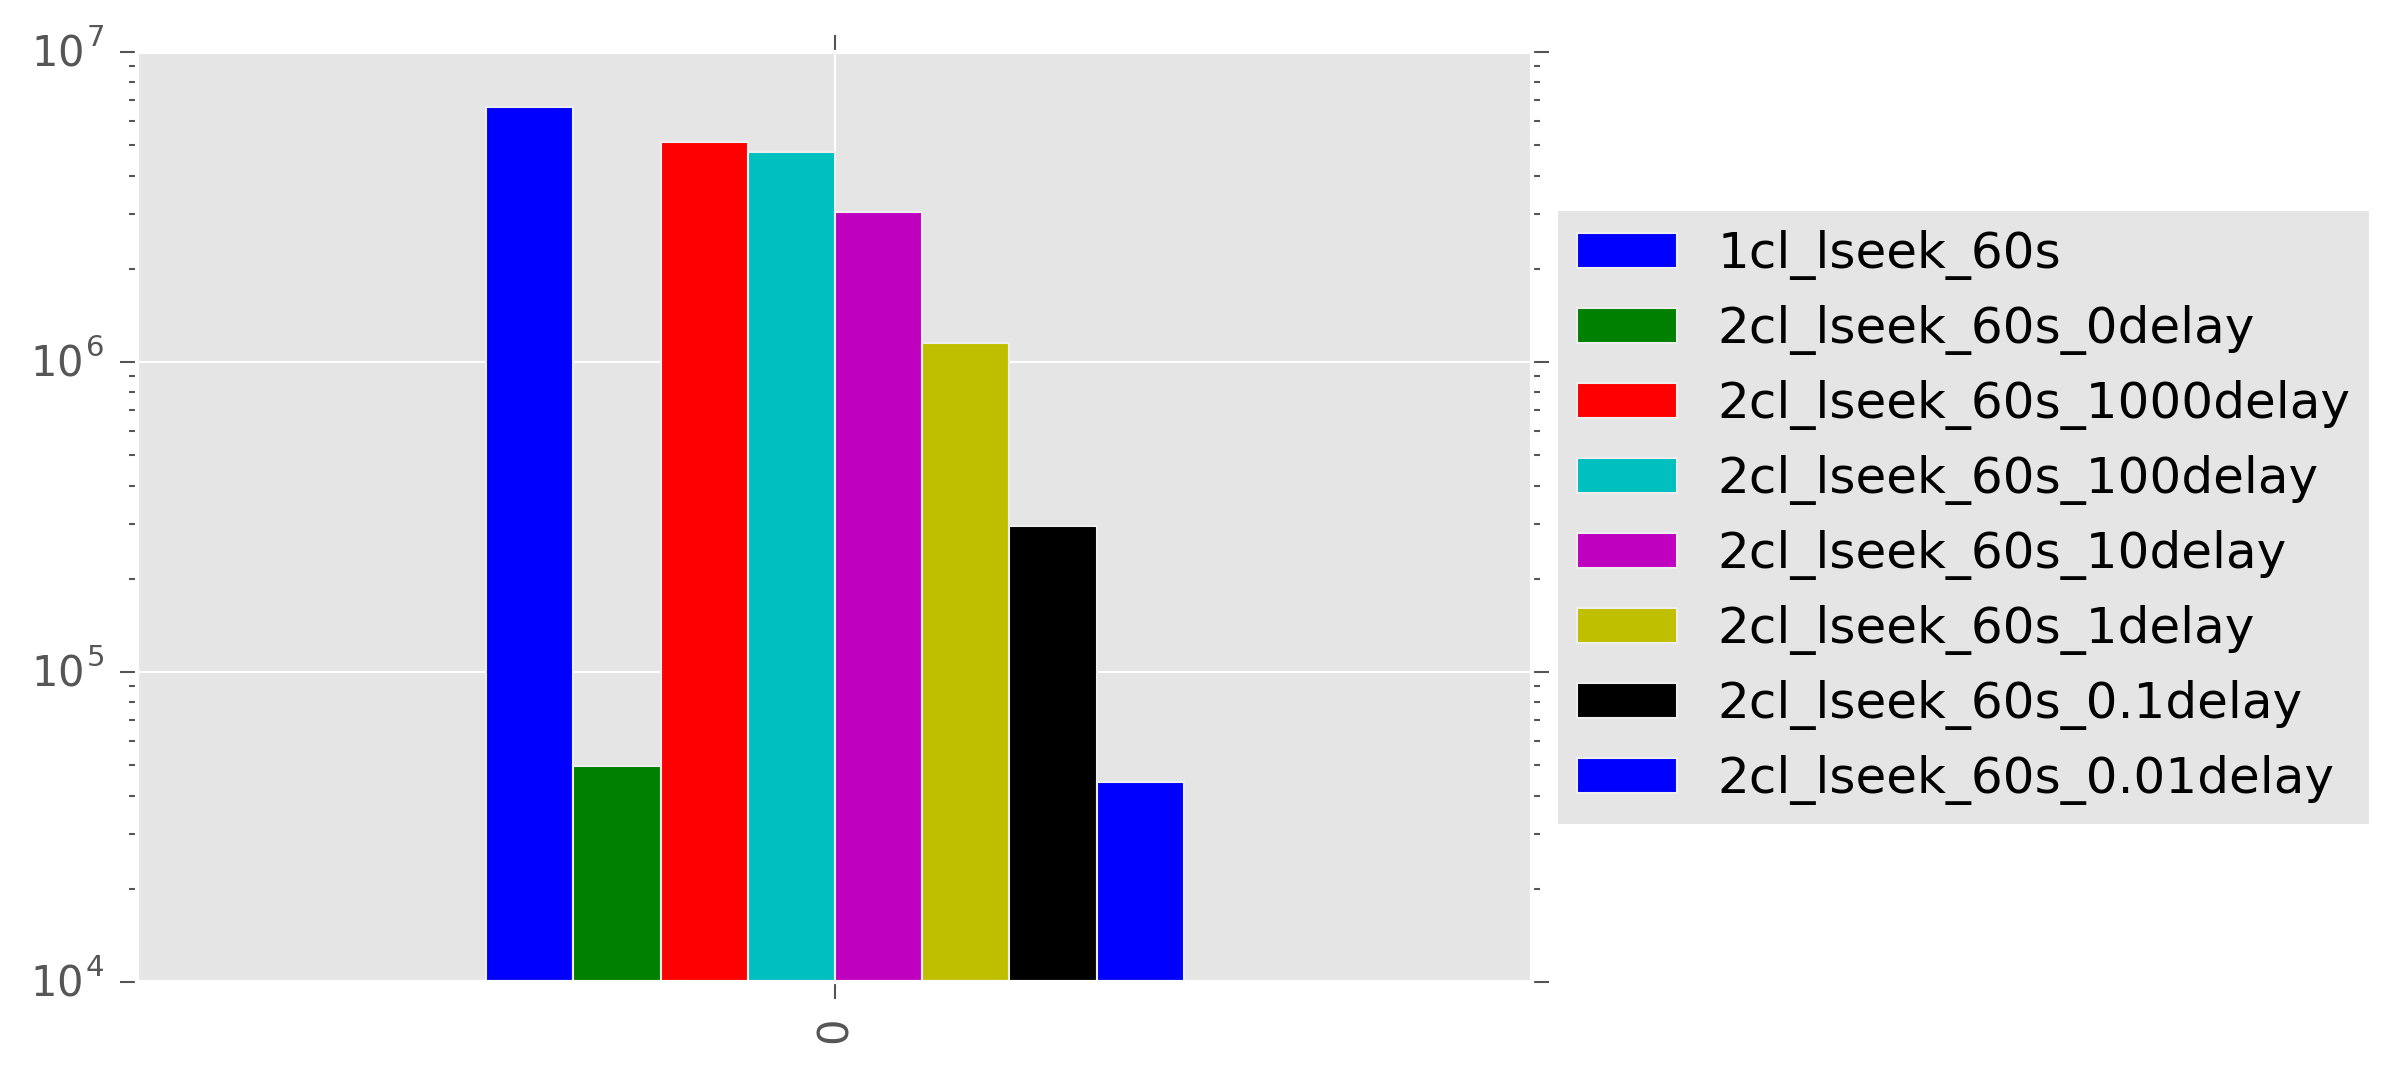
\includegraphics{figures/caps-delay-thruput.png} \caption{Forcing the client
%to drop their capabilities later (delay) improves throughput} \end{figure}
